\documentclass[a4paper,10pt]{article}
\usepackage[utf8]{inputenc}
\usepackage[margin=0.5in]{geometry}
\usepackage{amsmath}
\usepackage{xfrac}

\usepackage[T1]{fontenc}
\usepackage{textcomp}
\usepackage{listings}

\usepackage{graphicx}
\usepackage{wrapfig}
\usepackage{adjustbox}
\graphicspath{{figures/}}
\usepackage{hyperref}
\hypersetup{
    colorlinks,
    citecolor=black,
    filecolor=black,
    linkcolor=black,
    urlcolor=black
}

\usepackage [english]{babel}
\usepackage [autostyle, english = american]{csquotes}
\MakeOuterQuote{"}

%opening
\title{JAnalysisTools Manual}
\author{J. T. Smallcombe}
\begin{document}

\maketitle
\tableofcontents

\section{Introduction}
This library, designed to help working with root for analysis, contains several GUI analysis tools and useful sets of functions. An explanation of some of the major components is given here, but subclasses and functions will not be detailed.
Within the GUI classes hover over control to view explanatory tooltip text.
Various histogram presentation formatting and automated fitting macros (for spectroscopic peaks and detector efficiency curves) are also included and may be documented later. 

\section{Install}
This library has only been tested with ROOT6, it does not currently have any other non-standard dependencies.
Source the ROOT6 $thisroot.sh$.
In the base directory of the library run:
\lstset{language=bash}
\begin{lstlisting}
make clean
make -j4
source bin/thisjlib.sh
root -l bin/root_start.C
\end{lstlisting}
If all worked correctly, root started without error messages and is running with the library loaded.
For future use add a source of $thisjlib.sh$ to your bashrc and add $gSystem->Load("libJanalysistools.so")$ to your root startup script.

\section{jEnv Toolbar}
A graphical session manager toolbar to handle grabbing (selecting) of histograms without typing.
To create a new instance simply type:
\lstset{language=C++}
\begin{lstlisting}
new jEnv();
\end{lstlisting}
in a ROOT interactive session. A new window will open:
\renewcommand{\labelenumi}{\Alph{enumi}}
\begin{center}
\begin{tabular}{ c c }
\begin{minipage}{0.7\textwidth}
\begin{enumerate}
\item Open a the left panel mini file browser.
\item Grabbed Histogram Icon
\item Open a the peak fitting tab (copy grabbed histogram if \textit{TH1}), click the icon to start fitting environment in a new window.
\item Open the TSpectrumTool tab (if grabbed histogram is \textit{TH1}), click the icon to start fitting environment in a new window.
\item Create a new tab and draw a copy of grabbed histogram, click the icon to draw in a new window.
\item Overlay a copy of grabbed histogram in the \textbf{NEXT} canvas the user clicks.
\item Open a new 2/3D gating tool (if grabbed histogram is \textit{TH2/TH3}.)
\item Open a dialogue box to save grabbed object to disk.
\item Open a new TBrowser and draw grabbed histogram.
\item Close the toolbar.
\item Exit the ROOT session
\end{enumerate} \end{minipage}
&
\raisebox{-.5\height}{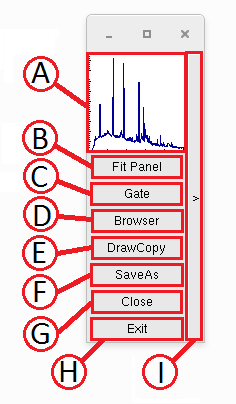
\includegraphics[width=0.23\textwidth]{jEnvA.png}}
\\
\end{tabular}
\end{center}

\subsection{Histogram Grabbing}
Whenever an instance of jEnv exists histogram grabbing is enabled in all $TCanvas$ instances, including those embedded in other classes/windows. Whenever a window containing a drawn histogram is clicked, a pointer to the first histogram of the frame is grabbed by jEnv and the small "Selected Histogram" icon will change. If a frame contains multiple histograms and you must click exactly on the desired histogram itself, not on the whitespace.

\begin{figure*}[!h]
\centering
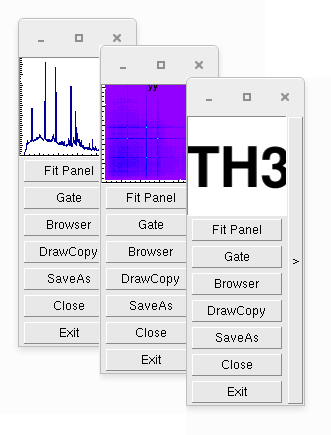
\includegraphics[width=0.3\textwidth]{jEnvB.png}
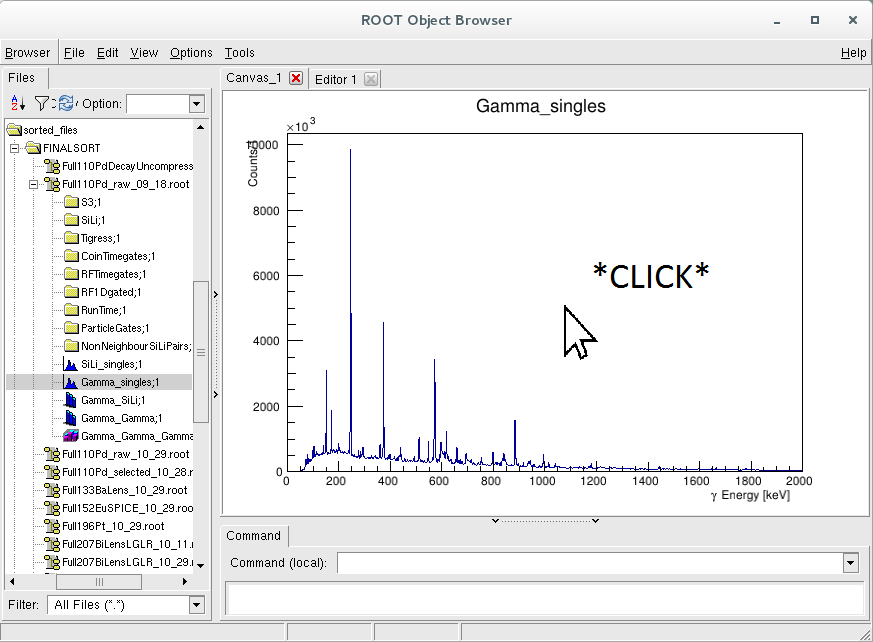
\includegraphics[width=0.52\textwidth]{jEnvD.png}     
\end{figure*}

Once a histogram is grabbed a copy of it will be passed to any of the functions of jEnv.

\newpage
\begin{wrapfigure}[14]{r}{0.25\textwidth}
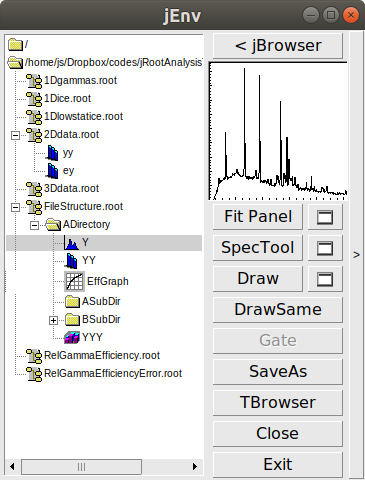
\includegraphics[width=0.25\textwidth]{jEnvE.png}
\end{wrapfigure}

\subsubsection{Histogram Lifetime}
A histogram can go out of memory scope in several ways. For speed, as grabbing is done on EVERY canvas click, only a pointer is stored. jEnv will refuse to do anything with its histogram pointer until it has established it is valid. To check if a histogram is still in memory jEnv checks the histogram against roots list of object, however this object search has limitations. If this histogram is still drawn in the same canvas that it was in when it was initially grabbed, then it will be found.

\subsubsection{Mini Browser}

The \textit{jBrowser} mini browser tab, hidden on the left hand side of the \textit{jEnv} toolbar, is a quick but (intentionally) limited browser.
The browser only shows system folders and .root files.
Only the \textit{TObjects} which \textit{jEnv} interacts with are visible within root files (currently histograms and graphs).
All functionality requires only a single click.
When \textit{TObjects} are selected they a passed to \textit{jEnv} from where you can select to draw, fit, gate etc.
 \textit{TH3} type objects can be easily passed to a gating tool without first drawing them, this is a distinct advantage over a standard TBrowser.
 Open files are handled by a global \textit{jTFileCustodian} so that files are closed only when all tools release them i.e. when a \textit{jEnv} instance is terminated open files are closed unless still in use by gating tool etc. 

\subsubsection{Environment Tabs}
Initially hidden on the right hand side of the jEnv are the environment tabs. Only the AddSubCompare tool tab is present initially. Fit panel, Spectrum tool and drawn objects will appear in subsequent tabs or can be explicitly drawn in their own windows by using the appropriate icon button.
The tabs can be shown/hidden by clicking on the long narrow button running along the side of the primary jEnv window.

\subsection{Histogram AddSubCompare Tool}
To the right side of jEnv is tab containing the AddSubCompare tool, this can be show/hidden by clicking the long button narrow button to the right of the primary jEnv window. The AddSubCompare tab is a simple tool to allow quick addition/subtraction and comparison of histograms from anywhere in the ROOT session.
Click either of the selected histograms windows $\alpha$ or $\beta$ to assign the currently grabbed histogram from jEnv, at this point a copy IS saved, not a pointer.

When the additions/subtraction function is selected the projected histogram is then given by $\alpha\pm \beta*f$ where \textit{f} is the fraction specified by the slider. 
In the case of scaled "ScaleAdd/Sub" the area of $\beta$ is first normalised to that of A. The resultant histogram can also be grabbed. The tool even allows combination of histograms with different binning, summing is done based on "user coordinates".
\textit{TH2}s may also be used, though only with identical binning. When using \textit{TH2}s a 4 second delay is enforced between updates.

Additional \textit{TH1} comparison modes have been added which overlay the two histograms, either with an adjustable scaling factor, or bin offset (Output histograms can be selected as new inputs to combine the two effects).

\begin{center}
\begin{tabular}{ c c }
\begin{minipage}{0.4\textwidth}
\begin{enumerate}
\item jEnv tab selection.
\item Selected Histogram $\alpha$ window/button
\item Swap inputs $\alpha$ and $\beta$
\item Selected Histogram $\beta$ window/button
\item Fraction $f$ text entry.
\item Change between functions.
\item Hide/Show error bars when drawing.
\item Fraction $f$ slider.
\item Result Window.
\item Show/Hide tabs panel.
\end{enumerate} \end{minipage}
&
\raisebox{-.5\height}{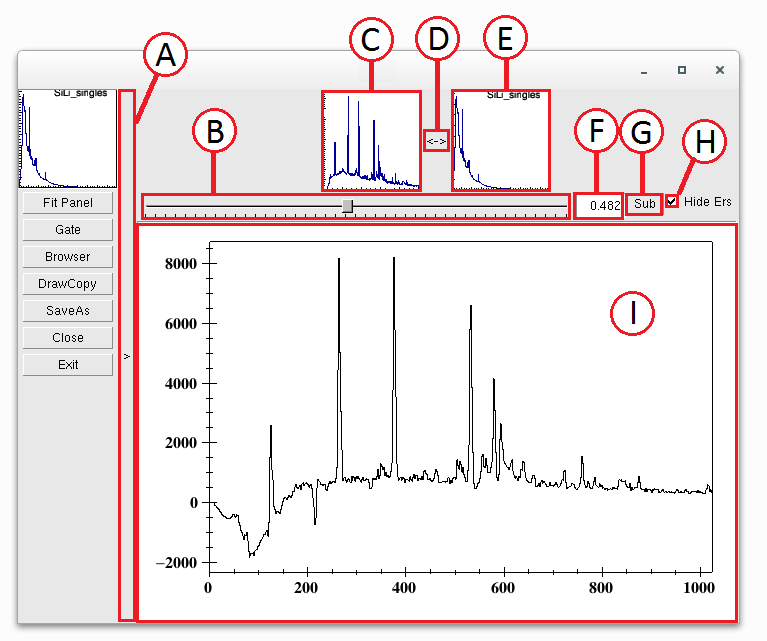
\includegraphics[width=0.55\textwidth]{jEnvC.png}}
\\
\end{tabular}
\end{center}

\newpage
\section{Gating and Background Subtraction Tool}
The gating tool is designed to provide live graphical gating and background subtraction for \textit{TH2} and \textit{TH3} histograms filled with any data. 
A new instance can be created from the jEnv toolbar or typing any of the following:
\lstset{language=C++}
\begin{lstlisting}
new jgating_tool();
new jgating_tool(TH2*);
new jgating_tool(TH3*);
new jgating_tool("HistogramName");
\end{lstlisting}
where "HistogramName" is the name (not title) of a histogram open in memory. The call with no arguments will grab the most recently selected or drawn histogram. If no valid input is found a window will not appear. Please wait a moment for the window to appear when using \textit{TH3}s, particularly if they are large.
\begin{center}
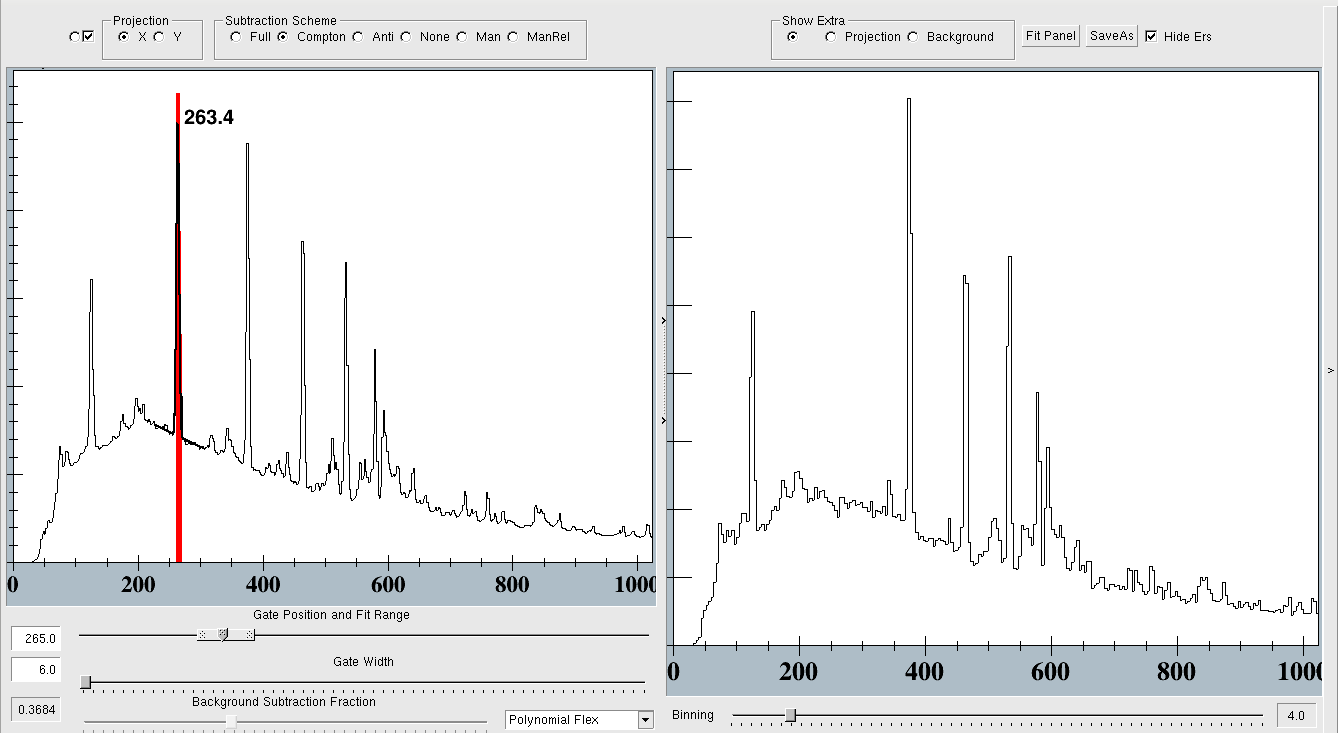
\includegraphics[width=0.55\textwidth]{toolA.png}
\end{center}

For a two dimensional histogram 2 panels are present. The leftmost is the "Gating Window" showing a projection on one axis of the histogram and the various gating controls. The rightmost is the "Result Window" containing the result of the gate and background subtraction.
For a three dimensional histogram a second "Gating Window" is present.

\subsection{Gating Window}

\begin{center}
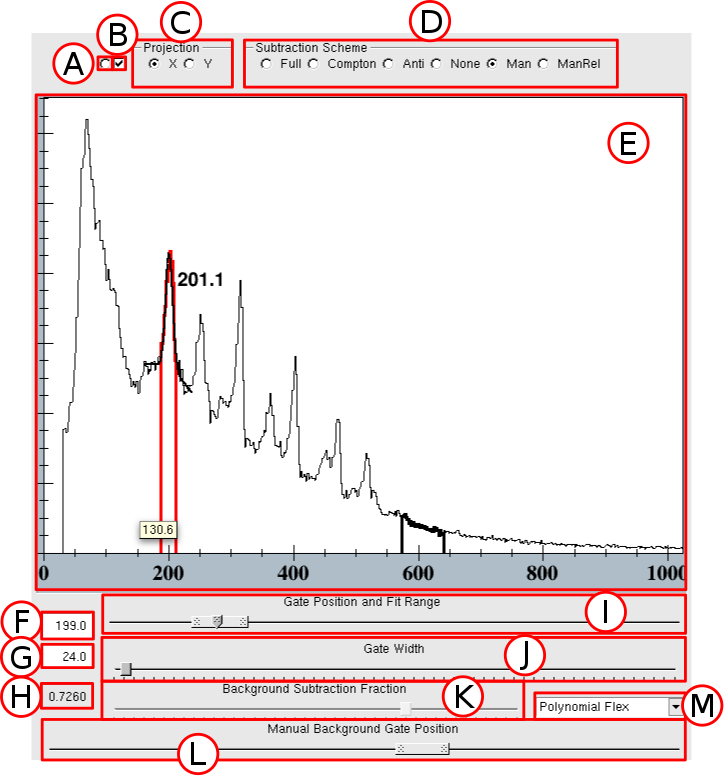
\includegraphics[width=0.5\textwidth]{toolB.png}
\end{center}
\begin{enumerate}
\item Overflow Peek - By default the shown projection excludes the overflow bins of the other axis. Hold this radio button to overlay the projection including overflow.
\item Show/Hide centroid marker - By default text is shown indicating the centroid of the peak when fitting options are used.
\item Axis Select - Change the axis on which gating performed. (USE TO RESET IF ERRORS OCCUR)
\item Background Subtraction Type (see section \ref{sec:subtype})
\item Projection Window - Window showing the current projection and gate, when appropriate shows also fit and background gate. You can double click in this window to move the gate.
\item Gate Centre - Operates as both a text entry box and readout for the slider. In user coordinates, but input will be rounded to nearest bin. 
\item Gate Width - As Gate Centre. 
\item Background Fraction Text Box - This can be used as a text entry box when manual background fraction mode is selected.
\item Gate \& Fit Slider - Use the central slider to adjust the position of your gate. When a fitting based background mode is selected, use the outer edges of the slider to adjust the range of the fit, relative to the gate position.
\item Gate Width Slider
\item Background Fraction slider - Can be used to manually adjust background fraction, when manual background fraction mode is selected.
\item Manual Background Gate - If manual background gate is selected, adjust the ends of this slider to define background gate (shown in black). This slider is hidden when not in use.
\item Background Fraction Mode -
Select how you would like to determine the background subtraction fraction, peak fit with fixed pol1 background, fit with auto-adjusting pol2 background, set manually OR use TSpectrum show background function (3 smoothing options pre-set).

\centering\raisebox{-0.9\height}{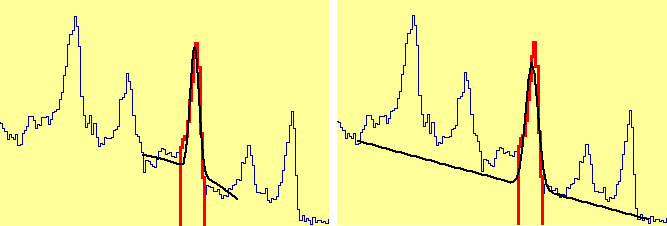
\includegraphics[width=0.5\textwidth]{jGateD.png}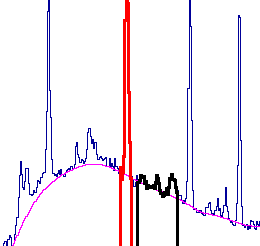
\includegraphics[width=0.25\textwidth]{toolC.png}}

\end{enumerate}

\subsubsection{Background Subtraction Type}\label{sec:subtype}
Depending on the nature of the data contained in the histogram and the the spectral quality in the region of the gate you may wish to define your background spectrum manually or in several other ways:
\begin{enumerate}
\item Full - This mode takes the full projection of the target axis as the background spectrum. A good first approximation in situations where a background cannot be clearly defined.
\item Compton - Background spectrum is formed by gating on the entire spectrum, including overflow, above the gate. Forms the best statistically sampled background spectrum for $\gamma$-ray gating. The background starts 2 bins above the gate, or 3$\sigma$ above the centroid (if a fit is used), whichever is greater. If directly adjacent to a spectrum dominating peak this may not be the best option. 
\item Anti - The background gate is the entire spectrum excluding the data gate. Appropriate for time gates.
\item None - No subtraction.
\item Man - User specified manual gate. When selected an additional slider will be displayed and the selected gate will appear in the gating window. If the background gate totally encompasses the data gate that region will be excluded (Enabling a background gate above and below).
\item ManRel - Relative position manual gate. As Man but the background gate will move when the data gate moves. Useful for scanning.
\end{enumerate}

\subsection{Result Window}
\begin{center}
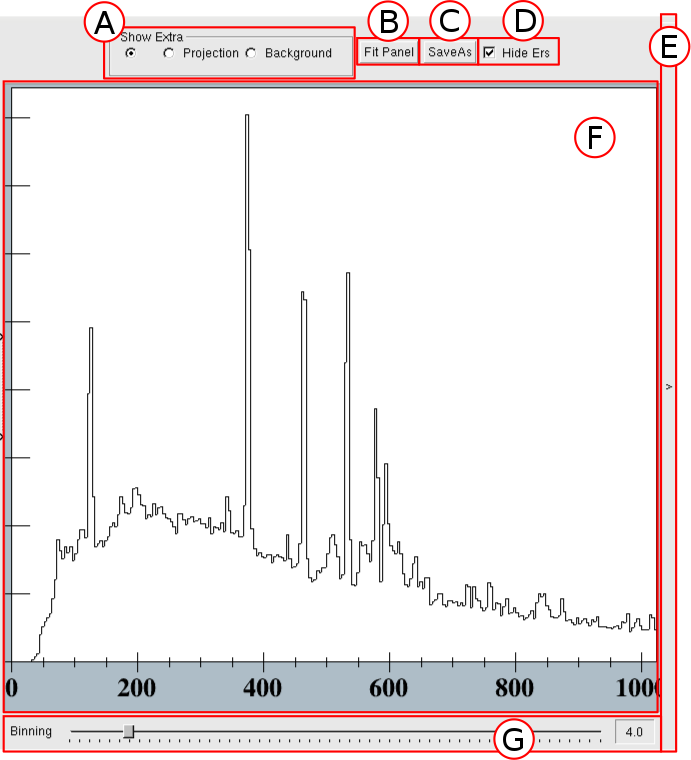
\includegraphics[width=0.5\textwidth]{toolD.png}
\end{center}
\begin{enumerate}
\item Draw Overlays - Show the total ungated-projection (scaled), or the currently subtracted background spectrum, overlain in the result window.
\item Open Peak Fit Panel - Open an instance of $UltraFitEnv$, the fitting tool is "connected" to the result canvas and will update with new input if the gate is changed. See Section \ref{sec:peakfit}.
\item SaveAs - Opens dialogue box to save the histogram currently drawn in the result frame to a file.
\item Hide Errs - Hide the error bars from background subtraction. \textit{Note: When selected fits performed with the ROOT FitPanel will not initially display, select the SAME drawing option to fix.}
\item Show/Hide Gate Summing Tool.
\item Result Frame. Double clicking in this window will perform a quick Gaussian fit at the cursor and display the centroid.
\item Rebin Result - Select a factor by which to rebin result histograms.
\end{enumerate}

\newpage
\subsection{Gate Summing Tool}
The Gate Summing Tool is used for saving the result histograms in memory after gating so that the results of multiple gates can be quickly summed.
\begin{center}
\begin{tabular}{ c c }
\begin{minipage}{0.6\textwidth}
\begin{enumerate}
\item Show/Hide Gate Summing Tool.
\item Create additional save slot.
\item Draw a sum of the selected histograms in a new window.
\item Delete all histograms in summing tool memory (Press twice).
\item Sum Check - Use the check marks to selected which saved histograms will be added to the output.
\item Save Buttons - Click to save/overwrite the current gating result histogram to a slot. The button will update with the centroid of the saved gate.
\end{enumerate} \end{minipage}
&
\raisebox{-.5\height}{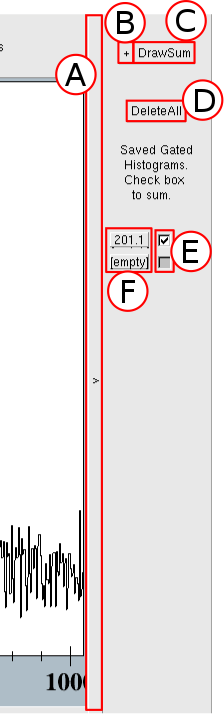
\includegraphics[width=0.15\textwidth]{jGateF.png}}
\\
\end{tabular}
\end{center}


\subsection{3D Gating Window}
For the first gate on a \textit{TH3} there is significant amount of computation so this is not done live. The output of the first gate is only performed when a new projection is selected, a different background mode is selected, or when the [Update] button is pressed.
\begin{center}
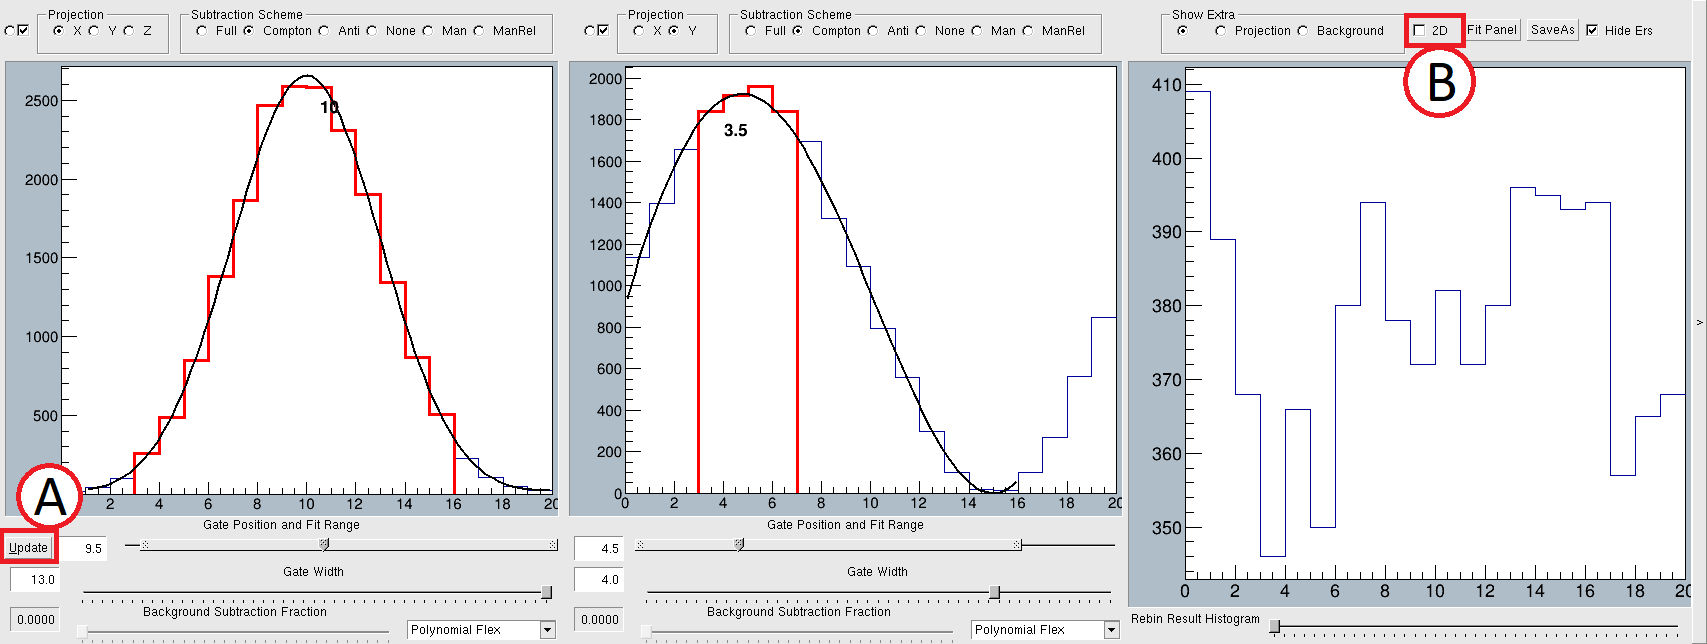
\includegraphics[width=0.95\textwidth]{toolE.png}
\begin{enumerate}
\item Update - Select after changing gate or background selections.
\item 2D - Do not perform a second gate but instead pass the \textit{TH2} result to the result frame. The gate sum tool can also be used in this mode.
\end{enumerate}
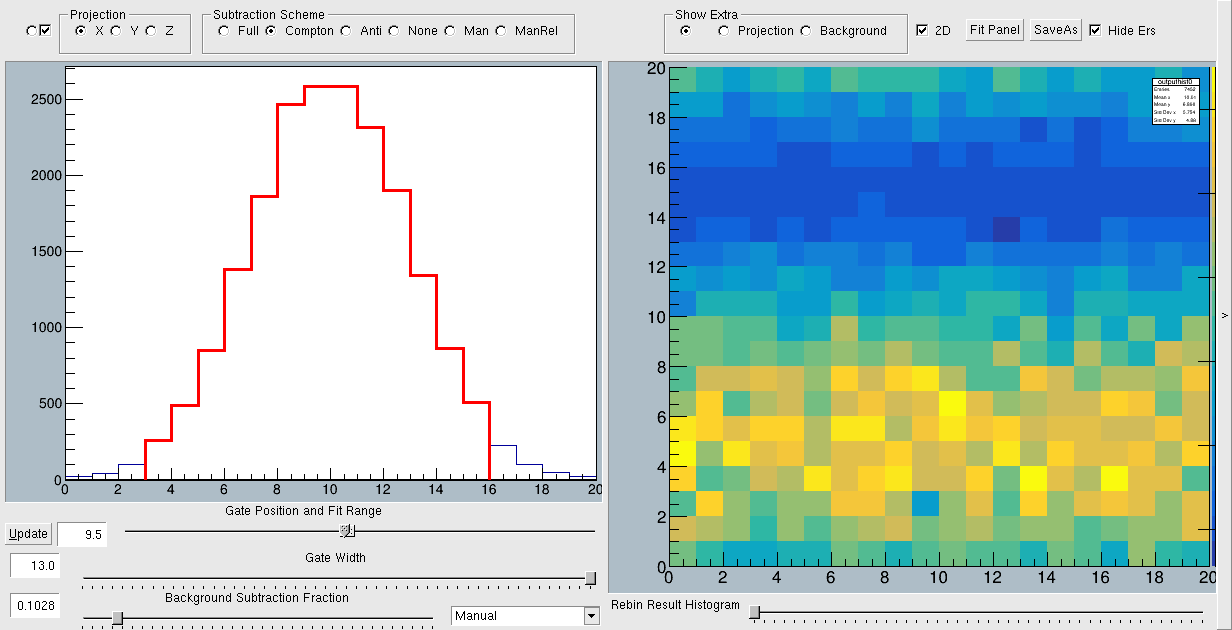
\includegraphics[width=0.6\textwidth]{toolF.png}
\end{center}

\newpage
\section{Peak Fitting Tool}\label{sec:peakfit}
\begin{wrapfigure}[8]{r}{0.4\textwidth}
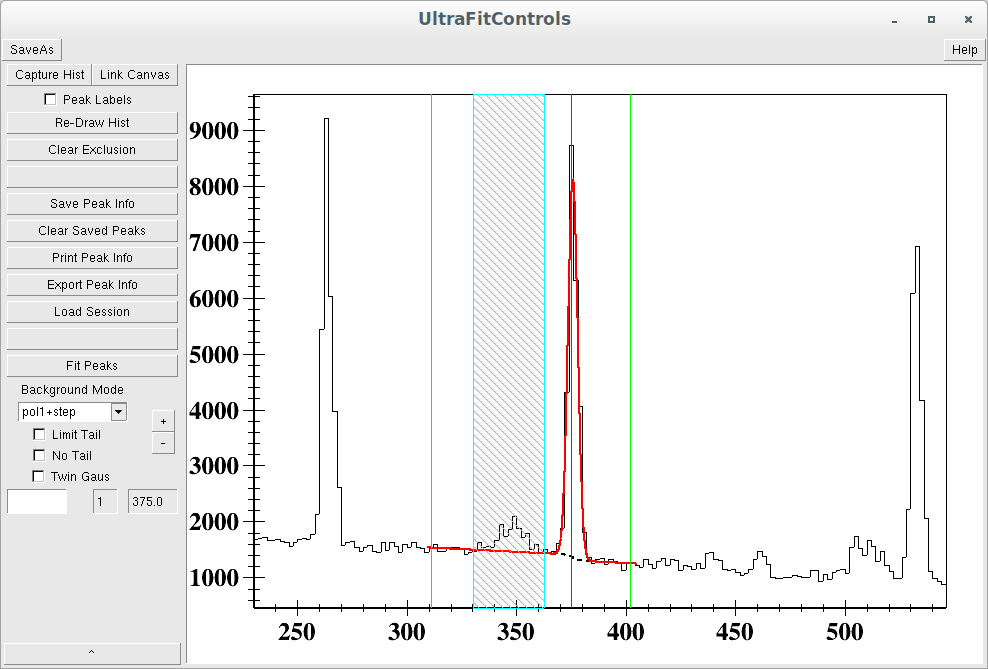
\includegraphics[width=0.4\textwidth]{jFitB.png}
\end{wrapfigure}
The UltraFitEnv fitting environment is designed for the automatic fitting of Gaussian peaks convolved with exponential tails.
The tool has some foibles that are absent from the root fitting environment, but it is far more tuned to the task of fitting spectra and saving the relevant data.
A new instance can be created from the jEnv toolbar or by typing one of the following in the root command line (with the appropriate substitution for relevant pointers):
\lstset{language=C++}
\begin{lstlisting}
new UltraFitEnv();
new UltraFitEnv(TH1*);
new UltraFitEnv(0,TCanvas*);
\end{lstlisting}
The tool operates in two primary modes:
\begin{itemize}
\item A histogram may be captured and stored by the tool.
\item A canvas can be linked to the tool, any new histogram drawn in that canvas will become the fitting target.
\end{itemize}

The fitting tool always stores an internal copy of the histogram which is the current fitting target. However, when the tool is "connected" it is to a selected canvas, not to a particular histogram. When a new histogram is drawn in the canvas the fitting tool updates it's internal histogram accordingly. Note: You cannot modify a histogram through the canvas the fitting tool is connected to (as the fitting tool performs \textit{DrawCopy} of it's internal histogram).

In order to begin fitting click either $[$Capture Hist$]$ or $[$Link Canvas$]$ and then immediately click on the Canvas/Histogram you want to fit

\subsection{Peak Fitting Toolbar}
Many of the functions of toolbar are duplicated by keyboard shortcuts.
\begin{center}
\begin{tabular}{ c c }
\raisebox{-.5\height}{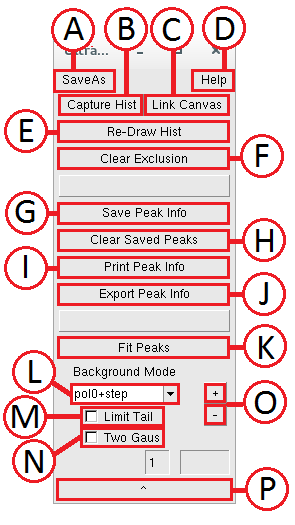
\includegraphics[width=0.3\textwidth]{jFitC.png}}
&
\begin{minipage}{0.70\textwidth}
\begin{enumerate}
\item Open dialogue box and save the current histogram to disk. Picture formats will include everything shown in the draw window, whereas .root files will only include saved fits.
\item Open help window.
\item Capture a subsequently selected histogram and draw a copy.
\item Connect the fitting tool to the subsequently selected canvas.
\item Show/Hide centroid labels of completed fits.
\item Re-Draw histogram and saved fits. (Reset problematic fit markers.)
\item Clear the user-defined exclusion regions.
\item Save the latest fit data to the in-memory list of confirmed fits. Fit will turn temporarily blue to confirm save.
\item Delete all saved fit data from memory (Press twice).
\item Print the in-memory confirmed fits data to the terminal.
\item Save the in-memory confirmed fit data to disk files peakinfo.dat and peakinfo.root. Use $[$SaveAs$]$ to specify the file name.
\item Open load dialogue to restore a session saved with "Export Peak Info".
\item Perform a fit with the current selection/inputs.
\item Change the background function of the fit.
\item Increase/decrease the number of peaks to fit.
\item Place fit constraints on tail shape parameters (Suitable for $\gamma$-ray spectra \& problematic fits), or use the more complex "Twin Gaussian" fit function (useful when fitting a sum of a small number of channels with differing resolutions).
\end{enumerate} \end{minipage}
\\
\end{tabular}
\end{center}

\newpage
\subsection{Peak Fitting Controls}
Click to select a peak for fitting, marker lines will appear showing the target peaks and fitting range. By default the nearest peak will be selected, press $[$ctrl$]$ to switch to exact bin selection. An automatic fit range will be shown, this can be overridden by clicking with the middle mouse button. To ignore bins containing anomalous features, create an exclusion region by pressing the $[Alt]$ and then clicking the first and last bins of the region. Note, using $[Re-Draw\;Hist]$ will clear exclusion regions.
\begin{center}
While the mouse pointer is over the fitting canvas the following controls and shortcuts may be used:

\begin{tabular}{ r l }
$[Left Click]$ & Select peak.\\
$[Ctrl]$ & Set manual bin select (default auto).\\
$[Enter]$ & Fit.\\
$[Middle Click]$ & Select fit-range.\\
$[Shft]$ followed by $[Left$ $Click]$ & Set fit-range marker.\\
$[Alt]$  followed by $[Left$ $Click]$x2 & Select exclusion region.\\
$[+]$ & Increase the number of peaks.\\
$[-]$ & Decrease the number of peaks.\\
$[0]$-$[9]$ keys & Set the number of peaks.\\
$[.]/[s]/[Del]$ & Save latest fit to list.\\
$[c]$ & Clear all exclusion regions.\\
\end{tabular}

If the controls do not seem to be working, it is likely a text-input box is still selected.
Look for the text cursor and click on an empty part of the environment to de-select the input box.
\end{center}
  
\subsection{Saving and Loading}
After completing fits there are 2 stages to saving. The first is to add the fit to the saved-fits list of the current session.
This is done with with the $[.]/[s]/[Del]$ keyboard shortcuts or the [Save Peak Info] button.
Any fits saved to the session list will be drawn in the result window by [Re-Draw Hist], printed to terminal by [Print Peak Info] and saved to disk by [Export Peak Info] or [SaveAs].  
\\
\\
When fits are saved to disk by [Export Peak Info] a plain text file peakinfo.dat containing the centroids, areas and errors is saved, along with a peakinfo.root file containing the full histogram and fit details in a format that can be loaded into root at a later date.
If peakinfo.dat exists in the current directory a terminal warning message will apear, click [Export Peak Info] to overwrite the file.
The [SaveAs] button at the top of a tool can be used to save an image file of the histograms and fits, or to save the current session with a user specified name rather than the default.
\\
\\
The [Load Session] button can be used to read a saved session root file which will overwrite any currently selected histograms, and the current session saved-fit list, with those from the file.
The [Clear Saved Peaks] button will clear the current session list and redraw the histogram with no fits, the button must be pressed twice to confirm the action (This has no effect on fit files saved to disk).

\subsection{Fit Function \& Logic}
The primary peak function consists of a pure Gaussian + an exponential convolved with a Gaussian, similar to Radware. The ratio is controlled by a sharing parameter that can take values from 0 to 1. An analytical normalisation is applied to the exponential peak such that its maximum value is always 1. After a fit the output data contains both a centroid and a "True centroid". The centroid is the maximum of the combined peak, the true centroid corresponds to the centroid of the pure Gaussian component which would correspond to the physical spectroscopic value.  
\\
\\
The tool is designed for fits over small energy regions, as such, all shape parameters of degenerate peaks are shared, as these parameters are dominated by energy dependant physical effects which do not change rapidly. Background across the fit region is approximated by a polynomial + an optional step function constrained by the peak parameters. The step should be used when peak sizes are large compared to background. Pol0, pol1 and pol2 backgrounds may be selected (pol2 are poorly constrained so a wider fitting region is needed).
\\
\\
For very small numbers of counts the fit mode will automatically switch to Poisson Likelihood fitting rather than Pearson Chi Squared minimisation. Exclusion regions will not function for Likelihood fitting.
\\
\\
A TwinGaus fit can be used when mixed resolution detector effects (such as Doppler shift) are significant. Each peak is fit with a narrow and a wide Gaussian with identical centroid. The background step is modified accordingly and all other fitting functionality remains the same. To avoid too many degrees of freedom the sigma ratio is highly constrained, also the relative proportion of the two Gaussian is fixed (default 0.6) and only allowed to vary if the Sharing parameter of the tail component is constrained or fixed (set to 1 to remove tail). The TwinGaus should only be used in the case of relatively isolated peaks.
\\
\\
Fit results will give two values for the area of each peak.
``Area.'' is calculated from the TF1 fit exactly.
``Int.'' is given as the difference between the histogram integral over a $\pm3\sigma$ range for each peak.
In the case of multiple overlapping peaks, the integral result is divided by the peak area ratios from the TF1 fit. 
An ``Err.'' marker at the end of the result line is shown when the 2 forms differ by more than 1$\sigma$ indicating a poor fit.
It is recommended to only take the ``Int.'' form result in the case of a single peak, or in situations in which a good background fit is achieved but peak shapes themselves are too irregular to be accurately fit.
The ``Int.'' results will not be calculated when exclusion regions are within the integration range.
\\
\\
Because this tool supports large exponential tails, the maximum value of the peak will often differ from the true spectroscopic centroid. In the case one wishes to specify the true-centroid this option can be selected in the shape parameter controls.

\subsection{Fit Inputs}
For multi-peak/degenerate fits, peak separations are specified, rather than absolute centroids. This provides more accurate fitting overall as it is less sensitive to small deviations in the absolute scale i.e. poor calibration. The area ratio between peaks may also be constrained if it is in known. When inputting multiple peaks to a fit, any constrained peaks should immediately follow the peak to which they are fixed. Un-constrained peaks should be in ascending order.
\lstset{language={},
  literate=~{$\sim$}2,
  upquote=true}
\begin{lstlisting}
Example: We have 3 peaks:
           An unknown ~130 keV, a known 125 keV and a known 145 keV.
           Inputs : A = 125
                    B = A + 20
		    C = 130
          -We set the tool for 3 peaks
          -Enter [20] in to the peak 0-1 "separation" input box.
          -Click on each peak A and C in the histogram window.
          -Click [Fit Peaks].
\end{lstlisting}
Note: When marking peaks in the fit canvas any peaks constrained to their neighbour do not need to be manually selected.
\\
\\
For both separation and area ratio between peaks, the box should be left blank to free the fit (centroids will have a default constraint). Uncertainties on both constraint parameters may also be added in the input box. If no error is given the parameter will be fixed. Only symmetric errors are currently supported. Plain text input is fairly robust and accepts ENSDF format errors:\\
Example inputs :\quad0.051\qquad0.051(2)\qquad0.051 0.002\qquad0.051+-0.002\qquad5.1E-2+2E-3
\label{sec:errors}
\\
\\
For problematic fits the shape parameters (Sigma, Decay and Sharing) may be constrained. The bottom-most button on the panel [$\wedge$] will expose these options. As with centroid \& ratio these parameters may be fixed or given with uncertainties and should be left blank when not constrained.
Alternately the Limit Tail check box applies preset limits on the tail parameters (Decay and Sharing) useful when fitting gamma spectra.
One may also select if true spectroscopic centroids are to be used as inputs or observed peak maxima.
\begin{center}
\begin{tabular}{ c c }
\raisebox{-.5\height}{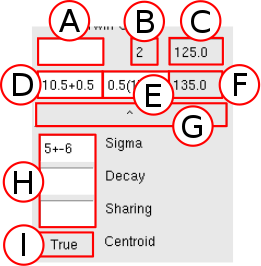
\includegraphics[width=0.3\textwidth]{jFitD.png}}
&
\begin{minipage}{0.7\textwidth}
\begin{enumerate}
\item Peak 0 centroid constraint input.
\item Number of peaks in fit.
\item Centroid of peak 0. Updated on selection or fit.
\item Fixed separation between peak 0 and peak 1.
\item Fixed size ratio between peak 0 and peak 1.
\item Centroid of peak 1. Updated on selection or fit.
\item Hide/Show fit shape parameter controls.
\item Fit shape parameter constraint inputs.
\item True/Maximum centroid inputs selection.
\end{enumerate} \end{minipage}
\\
\end{tabular}
\end{center}

\newpage
\section{TSpectrum Tool}
The $TSpectrum Tool$ provides a gui interface for manipulating \textit{TH1} spectra, correcting over-subtraction and subtracting continuum background with the ROOT $TSpectrum$ class.

\begin{center}
\begin{tabular}{ c c }
\begin{minipage}{0.35\textwidth}
\begin{enumerate}
\item Correct over-subtraction.  
\item Hide/Show bin errors.
\item Subtract TSpectrum background.
\item Flip histogram bin contents in X.
\item View/Result Window.
\item Rebin resultant histogram.
\item TSpectrum options.
\item TSpectrum smoothing iterations N.
\item Enable over-subtracted background.
\item Set minimum bin content to zero.

\end{enumerate} \end{minipage}
&
\raisebox{-.5\height}{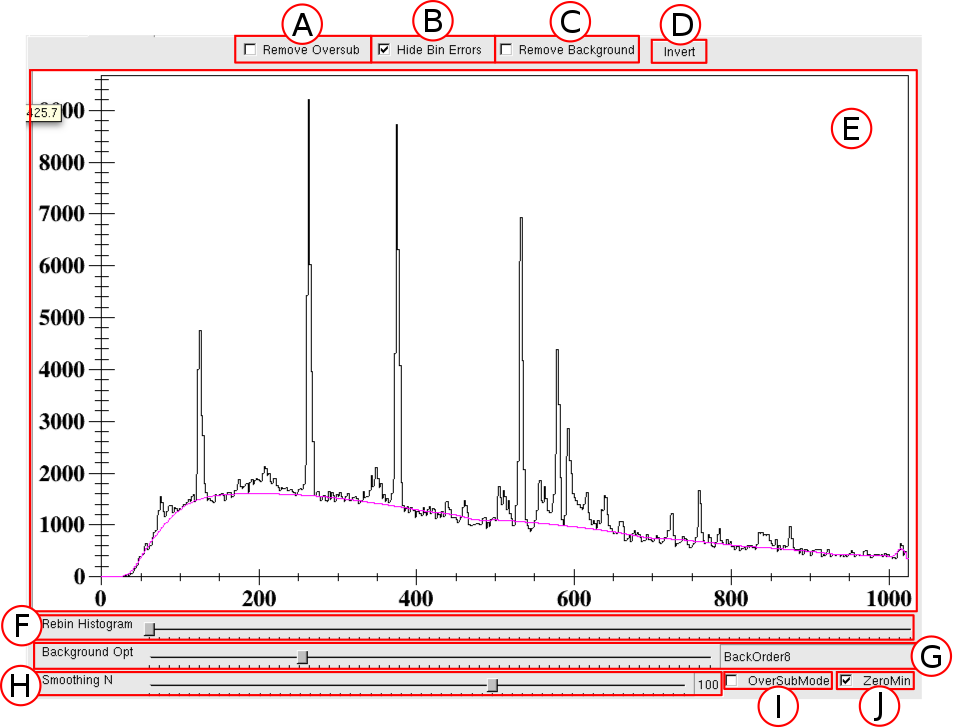
\includegraphics[width=0.65\textwidth]{TSpectrum1.png}}
\\
\end{tabular}
\end{center}

\subsection{TSpectrum Background}
This tool allows experimenting with the different settings of TSpectrum graphically.
One of the following options may be selected : $BackOrder2$, $BackOrder4$, $BackOrder6$, $BackOrder8$, $BackSmoothing3$, $BackSmoothing5$, $BackSmoothing7$, $BackSmoothing9$, $BackSmoothing11$, $BackSmoothing13$, $BackIncreasingWindow$, $Compton$. For details see the ROOT TSpectrum documentation. In general use the default $BackOrder2$ is sufficient and good agreement can be achieved with varying the number of iterations $N$. Occasional, in the case of over-subtraction, increasing to $BackSmoothing5$ or above may be needed. The $Compton$ option does not provide good background for a dense HPGe spectrum.
\\
When a good background is achieved you may elect to subtract it from the data with the $Remove Background$ tick button. Subtracting continuum background from TSpectrum is a matter of personal preference and is not scientifically rigorous. This can help fitting and automation.
\begin{center}
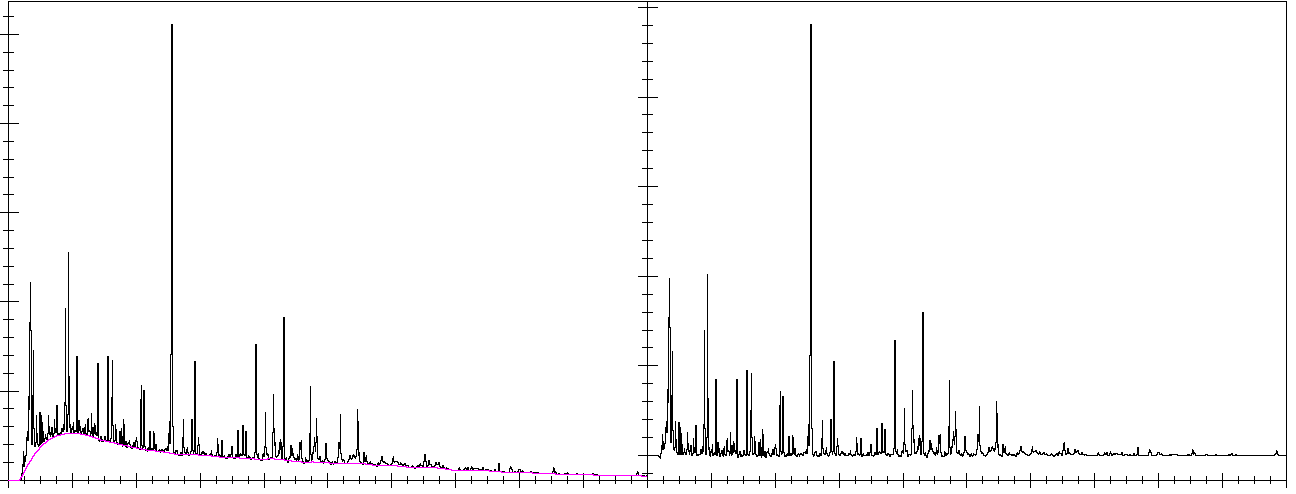
\includegraphics[width=0.5\textwidth]{TSpectrum4.png}
\end{center}

\subsection{Over-Subtracted Spectra}
The tool's provisional feature to correct over-subtraction is intended for situations in which spectra were produced such that over-subtraction was unavoidable. The default TSpectrum behaviour will fail in the presence of over-subtraction. Click the $OverSubMode$ option and the tool will attempt to compensate. Note that this option will produce backgrounds that are too high when over-subtraction is not present.
\begin{center}
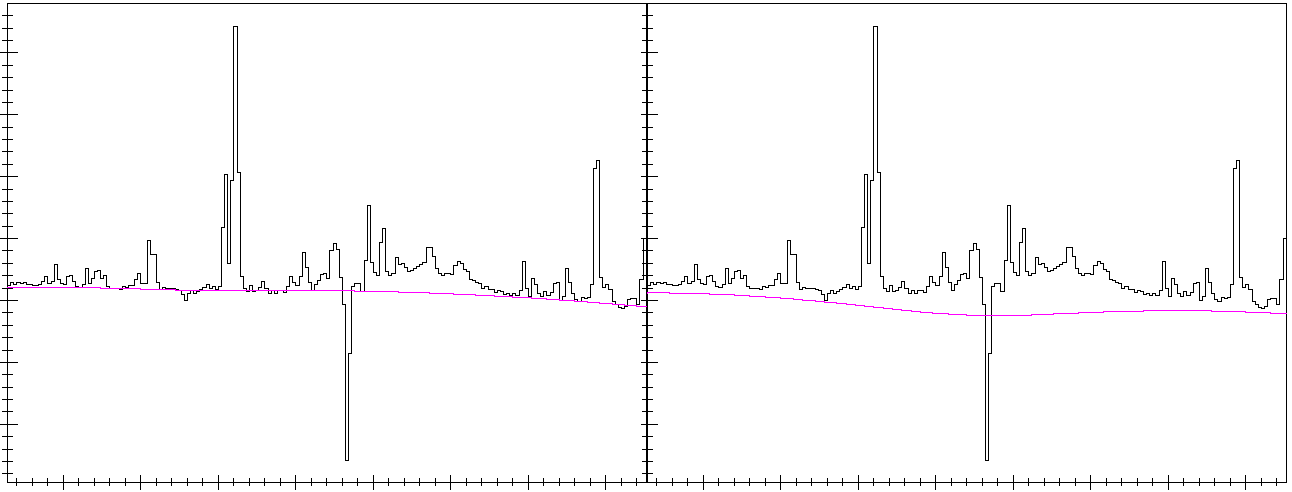
\includegraphics[width=0.5\textwidth]{TSpectrum2.png}
\end{center}
Additionally you may request to correct the over-subtracted histogram bins with the $Remove Oversub$ check box. Bins below the $TSpectrum$ line will be increased until they are within $1\sigma$. This is useful when one needs to the resultant spectra as a background for a subsequent subtraction, and you wish to avoid mistakenly \textbf{adding} counts. Ideally one would find an alternate original subtraction to avoid the problem in the first place, but when not possible this tool is intended to provide a possible solution, to be used with discretion when there is no alternative.
\begin{center}
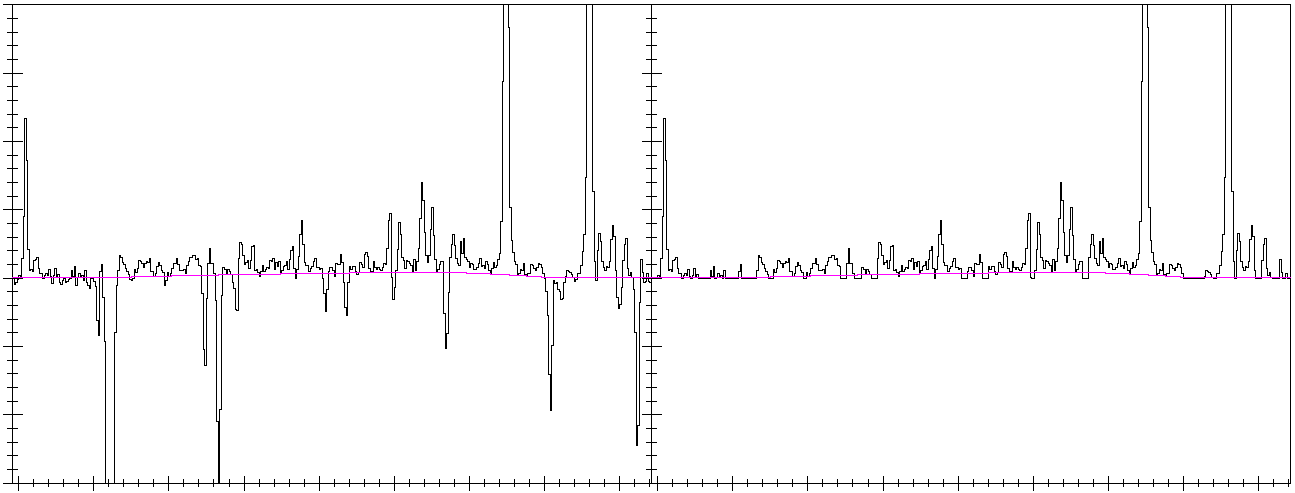
\includegraphics[width=0.5\textwidth]{TSpectrum3.png}
\end{center}
The $ZeroMin$ option simply sets that when performing a correction, no bin will be below zero. This accelerates the correction and is the default setting (irrespective of selection) when $Remove Oversub$ is selected but $OverSubMode$ is not.


\section{Command Line and Script Peak Fitting}
The following static function may be used to fit with Ultrapeak in scripts or on the command line:

\lstset{language=C++}
\begin{lstlisting}
FullFitHolder* Ultrapeak::PeakFit(
	TH1* HistogramToFit,
	double FitRangeLeft,
	double FitRangeRight,
	vector< jPeakDat > ListOfPeaks,
	int BackGroundMode = 0,
	int PeakType = 0,
	string SigmaParameterOveride="",
	string DecayParameterOveride="",
	string SharingParameterOveride="",
	TH1* ExclusionHistogram=0
);
\end{lstlisting}

The function returns a $FullFitHolder$ pointer. The pointer will =0 if the fit fails (so check!).
The \textit{FullFitHolder} class inherits from \textit{TF1}, so all \textit{TF1} functions may be called.
The calculated area of peak $i$ and it's error can be retrieved from the returned \textit{FullFitHolder} by calling:
\lstset{language=C++}
\begin{lstlisting}
ReturnedPointer->CVal(Ultrapeak::VPA(i));
\end{lstlisting}
and
\lstset{language=C++}
\begin{lstlisting}
ReturnedPointer->CVal(Ultrapeak::VPAe(i));
\end{lstlisting}
The centroids, "integral" and their respective errors can be fetched with $VPC$, $VPCe$, $VPI$ \& $VPIe$.


\subsection{PeakFit Function Inputs}

\renewcommand{\labelenumi}{\arabic{enumi}}
\begin{itemize}
	\item $ListOfPeaks$ consists of a $std::vector$ containing struct class $jPeakDat$ for each peak in the fit, see Section \ref{sec:jpeakdata} for details.
	\item $BackGroundMode$ can take the following values:
      \begin{enumerate}
      \setcounter{enumi}{-1}
      \item Constant background
      \item Constant + step under peaks
      \item Linear highly constrained by the fit range markers
      \item Linear
      \item Linear + step under peaks
      \item Quadratic
      \item Quadratic + step under peaks
      \end{enumerate}
    \item $PeakType$ can take the following values:
      \begin{enumerate}
      \setcounter{enumi}{-1}
      \item Gaussian + exponential tail
      \item Gaussian + small exponential tail
      \item Two Gaussians with identical centroid + one exponential tail
      \end{enumerate}
    \item $SigmaParameterOveride$, $DecayParameterOveride$, $SharingParameterOveride$ - these allow changing of the peak shape values from their defaults. Defaults are optimised for HPGe and Si(Li) spectra in keV. If used, provide a number in the string, the new value will be fixed in the fit. If desired include and uncertainty in the string (as explained in Section \ref{sec:errors}) to free the parameter
    \item $ExclusionHistogram$ should not be used in command line or script fitting.   
\end{itemize}

\subsection{jPeakDat}\label{sec:jpeakdata}
The jPeakDat struct holds the basic information needed to pass the fit function.
\lstset{language=C++}
\begin{lstlisting}
typedef struct jPeakDat{
	double Centroid;
	bool CentConstrained;
	double CentError;
	double Ratio;
	double RatioError;// <=0 fixed param
	jPeakDat(double c,bool cb=0,double ce=0,double r=0,double re=0):
	Centroid(c),CentConstrained(cb),CentError(ce),Ratio(r),RatioError(re){}
} jPeakDat;
\end{lstlisting}

Only centroid is required and it can be filled on construction. e.g.
\lstset{language=C++}
\begin{lstlisting}
	ListOfPeaks.push_back(jPeakDat(1432.2));
\end{lstlisting}

\begin{itemize}
\item $Centroid$ inputs in fitting are relative. The first peak centroid $ListOfPeaks[0].Centroid$ should be the absolute centroid, but for all other peaks $i>0$ the centroid should be relative, \\$ListOfPeaks[i].Centroid = centroid_i - centroid_{(i-1)}$
\item $CentConstrained$ tells the fit program is $CentError$ should be used
\item If $CentError\leq0$ the value of $Centroid$ will be fixed in the fit, else it will be given the range $\pm CentError$.
\item If $Ratio\leq0$ it is not used and the ratio of peak areas is not constrained in the fit, if a value is given it sets $area_i/area_{(i-1)}$ (it has no effect for peak 0).
\item  If $RatioError\leq0$ the value of $Ratio$ will be fixed in the fit, else it will be given the range $\pm RatioError$.
\end{itemize}



%\section{Histogram Formatting Functions}

\end{document}
